\chapter{Fluxo de envelhecimento de circuitos integrados}
\epigraph{\textit{Open your mind to what I shall disclose, and hold it fast within you; he who hears, but does not hold what he has heard, learns nothing.}}{-Dante Alighieri}
Um dos pontos mais importantes para a simulação e obtenção de dados que deem apoio às futuras pesquisas e projetos é a decisão de quais soluções técnicas, das disponíveis, será utilizada para obter resultados coerentes com experimentos reais. Este é um ponto crucial deste trabalho pois os dados obtidos e o comportamento observado devem dar apoio à tomada de decisões por parte de sistemas que atuam na recuperação de falhas.

Para garantir esta fidelidade, foi escolhida a ferramenta Relxpert$^{\textcopyright}$. Este simulador é desenvolvido especialmente para cálculo de envelhecimento de circuitos integrados e considera efeitos como HCI, TDDB e NBTI/PBTI. Dada à experiência e proximidade da Cadence com o mercado de semicondutores, temos disponível uma ferramenta confiável para simulação e extração de resultados.

Outro fator importante é o uso de parâmetros de envelhecimento coerentes com os dispositivos reais. Ao evitar a modelagem destes parâmetros (e da criação de modelos para os efeitos de HCI, TDDB e BTI) é possível integrar a solução aqui apresentada a qualquer modelo. Como resultado, é proposta uma solução independente das ferramentas escolhidas, da tecnologia empregada e da metodologia utilizada no cálculo dos parâmetros.

Para nossa conveniência, utilizamos parâmetros disponibilizados pela própria ferramenta e que se assemelham às tecnologias de 90nm empregada pelas \textit{foundries} de dispositivos semicondutores.

\section{Estratégia do fluxo}
\label{section_estrategia_fluxo}
O fluxo de envelhecimento para extração é composto de seis etapas principais sumarizadas abaixo e representadas na figura \ref{figure:fluxo_geral}:
\begin{enumerate}
	\item Criação de uma tabela com condições ambientais pré-estabelecidas;
	\item Identificação de um caminho crítico para análise e criação de uma \textit{netlist} primitiva;
	\item Envelhecimento da \textit{netlsit} primitiva e criação de uma envelhecida;
	\item Simulação da netlist envelhecida;
	\item Extração dos atrasos relativos e do MTTF;
	\item Criar e popular um BDPE.
\end{enumerate}
\begin{figure}[H]
\center
{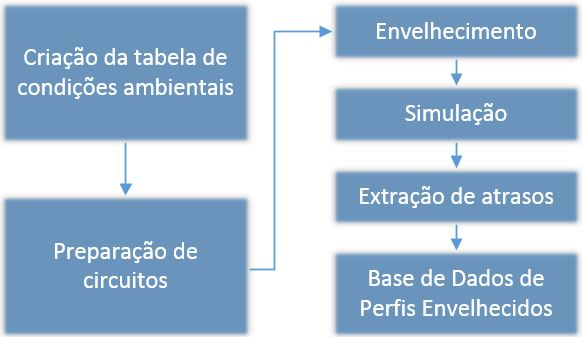
\includegraphics[width=0.7\textwidth]{images/fluxo_geral}}
\caption{Fluxo geral utilizado no envelhecimento de circuitos integrados.}
\label{figure:fluxo_geral}
\end{figure}
É importante salientar que esta é apenas uma das forma de se popular a base de dados de perfis envelhecidos, conforme mencionado na seção \ref{section_visao_geral}, e pode ser utilizada em conjunto com as demais técnicas mencionadas na seção. Para este trabalho, esta tabela de condições ambientais servirá um duplo propósito: representar o BDM e o BDPE. No capítulo 5 é detalhado como esta tabela é utilizada na criação dos modelos de predição de MTTF.

A simulação \textit{offline} do sistema a ser observado (ou de parte dele) exige algumas \textit{entradas} a serem utilizadas no fluxo de envelhecimento:
\begin{enumerate}
\item Um conjunto de netlists a serem envelhecidas. Neste trabalho são utilizadas netlists cuja sintaxe é \textit{Spectre};
\item Os arquivos de modelos para os dispositivos do tipo nMOS e pMOS. Estes arquivos contém não somente os parâmetros de operação como também os de envelhecimento;
\item Uma tabela de condições ambientais a serem aplicadas ao sistema. No trabalho foram utilizados os modelos BSIM4 \cite{Karl2008}.
\end{enumerate}
Como \textit{saída} são obtidos:
\begin{enumerate}
\item Uma netlist com cada parâmetro de envelhecimento que será usado na simulação envelhecida;
\item Dados de simulação da netlist envelhecida e atrasos relativos à uma saída pré-determinada.
\end{enumerate}

Durante este processo de envelhecimento, etapas intermediárias são necessárias, conforme mostrado na figura \ref{figure:fluxo_ferramenta}:
\begin{enumerate}
	\item Cálculos de envelhecimento: etapa onde são obtidas as variações de parâmetros dos dispositivos empregados e como degradam com o tempo. Além disso, uma netlist ``pré-processada'' é criada. Isso significa que ela já foi modificada com as condições ambientais necessárias para a simulação envelhecida mas sem as informações de degradação dos dispositivos que a compõe. Estas mudanças são retiradas dos arquivos de modelo e informam como a tensão de limiar $V_{TH}$ de um transistor nMOS, por exemplo, aumenta com o decorrer do envelhecimento. 
	\item Degradação de transistores: a ferramenta envelhece os dispositivos e anexa estas informações em um ou mais arquivos de modelos. Esses arquivos são atualizações baseadas nas informações originais e possuem novos valores para alguns parâmetros (\textit{p.ex.} tensão de limiar). Estes dispositivos são atualizados de forma a refletir quais serão os valores destes parâmetros após um certo período de tempo. Exemplo: considere que, em seu estado original, um dispositivo nMOS possui um $V_{TH}=1.1V$. Após simular dois anos de envelhecimento para sistema, seus transistores nMOS passam a precisar de $V_{TH}=1.23V$. Este incremento de 0.13V é consequência da degradação do sistema ao longo desses 2 anos. 
\end{enumerate}

\begin{figure}[H]
\center
{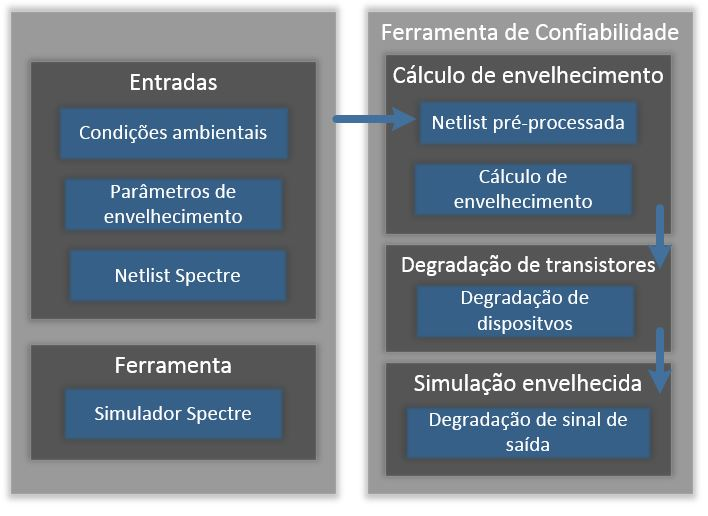
\includegraphics[width=0.7\textwidth]{images/fluxo_ferramenta}}
\caption{Entradas e saídas da ferramenta de envelhecimento.}
\label{figure:fluxo_ferramenta}
\end{figure}
Estas etapas de cálculo são realizadas pela ferramenta de envelhecimento e são ``transparentes''. Isso significa que não há, normalmente, uma intervenção por parte do projetista sobre estes cálculos, que seguem os modelos da própria ferramenta e os parâmetros de tecnologia fornecidos pela fabricante. É possível, entretanto, analisar quais mudanças e resultados são inseridos nos diversos arquivos utilizados pelos simuladores.
\section{Implementação do fluxo e integração com as ferramentas de envelhecimento}
\label{section_implementacao}
As seções seguintes irão descrever as etapas necessárias para a criação e integração do fluxo com as ferramentas e a metodologia apresentada no capítulo 3. São dados mais detalhes da preparação das \textit{netlists}, dos perfis de envelhecimento e da análise dos caminhos críticos.
\subsection{Preparação de células lógicas e netlists}
\label{subsection_celulas}
Para representar o comportamento de um sistema são, por vezes, utilizadas \textit{netlists}, que são arquivos cuja função é descrever como um sistema ou diversos componentes eletrônicos se interconectam. A netlist pode conter fios, pinos, parâmetros elétricos, regimes de operação (\textit{p. ex. temperatura, tempo de envelhecimento}), diretivas de simulação, referência a modelos de transistores, fontes de tensão e corrente, lógica booleana, entre outras informações.

Entretanto é preciso diferenciar as netlists geralmente disponíveis em um projeto de circuitos digitais:
\begin{enumerate}
	\item descrição comportamental: utilizando-se de uma linguagens de descrição de hardware (HDL), especificam o comportamento de um sistema. A descrição é de \textit{alto nível}, não contendo detalhes de quais portas lógicas são utilizadas para implementar a lógica desejada;
	\item descrição estrutural: ainda utilizando HDL, descreve uma lógica através da interconexão entre portas lógicas;
	\item descrição esquemática: detalha a interconexão entre os transistores além de possuir informações sobre fontes de alimentação, fios, elementos capacitivos, modelos de transistores, temperatura de operação e qualquer outra informação necessária para a simulação dos circuitos descritos.
\end{enumerate}

Para o fluxo aqui apresentado é proposto a utilização de uma netlist esquemática pois, por possuir a descrição dos transistores, pode conter também os parâmetros de degradação dos mesmos. Entretanto, caso o projetista não possua o esquemático, é possível obtê-lo através de uma descrição comportamental ou estrutural. Para isso, um processo de síntese ou tradução é realizado com o auxílio de softwares de \textit{projeto de circuitos integrados} (\textit{i.e.} Electronic Aided Design, EAD). Por síntese entende-se o processo de interpretação da descrição de alto nível de um circuito ou conjunto de circuitos e tradução para uma representação de portas lógicas. Define-se por tradução como sendo o processo de representar uma netlist estrutural em uma esquemática.

Caso o ponto de partida seja uma descrição comportamental, uma netlist estruturada é obtida por síntese e em seguida uma netlist esquemática. Em uma descrição comportamental não existe informação de quais portas lógicas são utilizadas, apenas as funcionalidades do sistema. Como as portas são desconhecidas, não é possível determinar quais transistores serão utilizados e, consequentemente, como os efeitos de degradação afetam os mesmos. Posteriormente, a descrição estrutural será traduzida para uma esquemática contendo todos os transistores necessários para implementar as funcionalidades projetadas.
 
Essa tradução necessita de uma biblioteca de portas lógicas que, por sua vez, possui informações detalhadas de como elas são implementadas para uma determinada tecnologia de um fabricante específico. Esta biblioteca é fornecida pelas \textit{foundries} e sua descrição detalhada foge do escopo deste trabalho. O fluxo proposto assume que a implementação destas portas já está disponível e que é possível sintetizá-las, separadamente ou em conjunto, para que uma netlist seja gerada.

Para a utilização de um sistema no fluxo que está sendo proposto é mister identificar como ele está descrito (descrição comportamental, estrutural ou esquemática) e obter gradativamente, quando necessário, a netlist esquemática.

\subsection{Preparação dos perfis de envelhecimento}
\label{subsection_perfis}
O circuitos integrados atuais trabalham sobre condições de operação que oscilam constantemente. Podemos abordar estas variações de inúmeras maneiras. Entretanto, esse trabalho considera duas abordagens complementares que propõem interpretar as variações de duas maneiras:
\begin{enumerate}
	\item Para um intervalo de tempo $t$, as variações são sumarizadas como as médias das tensões aplicadas e temperaturas medidas no dispositivo ao longo desse tempo. Isso significa que, se um sensor $S_{V,1}$ registrou uma média de $1.1V$ e um outro $S_{T,1}$ registrou uma média de $45^{o}C$, aquele intervalo será caracterizado por $V_{conj,1}=1.1$ e $T_{conj,1}=45$;
	\item Um perfil de envelhecimento representa um conjunto de intervalos (ou faixas) sob os quais o sistema esteve submetido ao longo de sua operação, conforme mostrado na figura \ref{figure:profile_sets}. Ao se variar a quantidade de tempo sob qual o circuito permanece em cada elemento deste conjunto, obtemos uma tabela que possui um sumário das condições ambientais impostas ao sistema.
\end{enumerate}
Assim sendo, existe uma tabela que associa variações de temperatura e tensão a um ciclo de vida de um sistema. Cada variação dos parâmetros de tensão de alimentação $V_{DD}$ das portas lógicas e da temperatura $T$, é associada a um tempo de operação, conforme exemplificado na tabela \ref{tb:BDPE_reduzida}. A definição dos valores $p_{T(w,x)}$ e $p_{V(w,y)}$ e da quantidade de conjuntos $T_{conj,X}$ e $V_{conj,Y}$, descritos na tabela \ref{tb:BDPE}, influencia diretamente na precisão das simulações a serem realizadas.

Para exemplificar, consideremos um sistema analisado durante 1 ano cujos perfis de operação são sumarizados pela tabela \ref{tb:regressao_multipla_exemplo2} abaixo:
\begin{table}[H]
	\centering
	\caption{Tabela de exemplo utilizada para o cálculo das variações de perfis.}
	\begin{tabular}{@{}l|l|l|l|l@{}}
		\toprule
		30 & 50 & 1.0 & 1.1 & MTTF \\ \midrule
		13 & 1 & 12 & 2 & 1.2 \\
		7 & 7 & 9 & 5 & 2.0 \\ \bottomrule
	\end{tabular}
	\label{tb:regressao_multipla_exemplo2}
\end{table}

Para o primeiro registro, o sistema fica submetido a $T_{conj,1}=30$ e $T_{conj,2}=50$ durante 1 ano. Entretanto, $T_{conj,1}=30$ influencia o sistema por mais tempo, pois possui um valor de $p_{T(w,x)}$ maior. Somando-se os valores de $p_{T(w,x)}$ para ambos os conjuntos de temperatura, o sistema é descrito como tendo sido submetido a uma temperatura média de $30^{o}C$ treze vezes ao longo de 1 ano e somente uma vez à temperatura média de $50^{o}C$, totalizando 14 intervalos de tempo $\Delta t$.

Desta forma, para um tempo de simulação $t_{sim}$ e $N$ intervalos, cada $\Delta t$ corresponde a um período de tempo dado por:

\begin{equation}
\Delta t = \frac{t_{sim}}{N}
\end{equation}

No exemplo acima $\Delta t\approx 0.07$ anos. Caso o sistema seja representado pelo BDPE da tabela \ref{tb:BDPE_reduzida}, por exemplo, seu perfil possui então $N=50$ intervalos distribuídos entre 5 conjuntos de médias de temperatura e tensão de alimentação, tornando o perfil mais granular. Como é necessário representar o mesmo sistema em diferentes intervalos de tempo, e cada intervalo pode ter suas próprias condições ambientais, o fluxo necessita de $N$ representações esquemáticas.

Essa granularidade altera a quantidade de etapas necessárias para o fluxo, conforme representado na figura \ref{figure:fluxo_detalhado}:

\begin{figure}[H]
	\center
	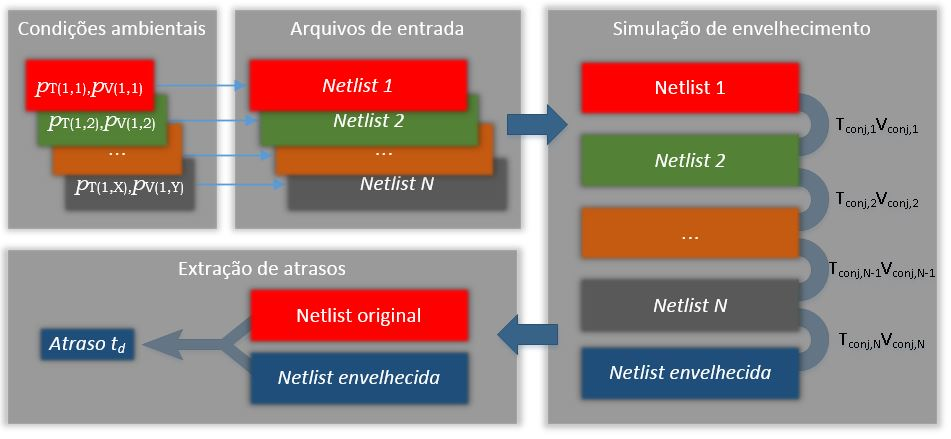
\includegraphics[width=1\textwidth]{images/fluxo_detalhado}
	\caption{Detalhamento do fluxo de criação, modificação e extração de resultados.}
	\label{figure:fluxo_detalhado}
\end{figure}

Cada uma das $N$ condições ambientais, representado no bloco \textit{condições ambientais} da figura \ref{figure:fluxo_detalhado}, será utilizada na criação de $N$ netlists, cada uma com seus respectivos $p_{T(w,x)}$ e $p_{V(w,y)}$. A degradação é realizada em $N$ etapas ao longo de um tempo $t_{sim}$, onde cada netlist é degrada durante um intervalo $\Delta t$.

Para o exemplo da tabela \ref{tb:regressao_multipla_exemplo2}, se o sistema estiver sendo observado durante 1 ano, a \textit{netlist 1} estará submetida à $T_{conj,1}=30$ e $V_{conj,1}=1.0$ durante $0.07$ anos na primeira etapa. A \textit{netlist 2} é criada e alterada com as novas condições (que para este exemplo são as mesmas), que também prevalecerão durante $0.07$ anos. Esse processo se repete até que todas as $N$ netlists sejam criadas.

Dado o exposto anteriormente, o projetista precisa preencher o BDPE com dados que provem de simulações, testes de estresse ou extraídas de campo. Neste trabalho os BDPEs foram preenchidas com dados de simulação exclusivamente e os valores de $p_{T(w,x)}$ e $p_{V(w,y)}$ foram gerados aleatoriamente, por conveniência. Essa escolha pode obedecer uma distribuição normal, caso seja adequado. A metodologia aqui proposta é indiferente quanto à essa escolha.

\section{Extração de caminhos críticos}
\label{section_extracao_caminhos}
Todas as descrições esquemáticas geradas na seção \ref{subsection_perfis} são simuladas uma após a outra. Entretanto, representar cada transistor de um sistema pode ser impraticável. Isso se deve ao fato de que os processadores mais recentes possuem bilhões de transistores \cite{Alcorn2016}, tornando a etapa de degradação de todos eles inviável e computacionalmente custosa. Além disso, para uma simulação adequada, é necessária a ativação de todas as entradas do sistema, o que também pode ser impeditivo.

Para mitigar este problema, é possível se realizar a análise temporal estática do \textit{pior caminho} de um sistema, sendo considerada uma técnica conservativa e bem estabelecida, apesar de não ser a mais moderna \cite{Orshansky2002}. O \textit{pior caminho} representa o trecho condutivo mais crítico ao sistema, onde qualquer violação de temporização torna a operação do sistema não confiável.

Dessa forma, realizar a degradação do caminho crítico é uma abordagem vantajosa e mais realística pois obtém uma quantidade reduzida de transistores e entradas a serem ativadas. Um problema desta abordagem é que não há garantia de que, após a degradação, este caminho continue sendo o mais crítico. Para mitigar este problema, mais de um caminho pode ser utilizado e posteriormente selecionado como pior aquele cuja atraso seja o maior.

A extração dos caminhos críticos é realizada pelas próprias ferramentas de EDA, que são capazes de reportar quantos caminhos forem desejados pelo projetista, gerar uma descrição esquemática e criar fontes de alimentação que ativem os piores caminhos.
\section{Simulação e degradação}
\label{section_simulacao}
Uma vez criadas as netlists e o BDPE, a degradação é realizada de fato. Foram realizadas as etapas dos blocos de ``condições ambientais'' e ``Arquivos de entrada'' representados na figura \ref{figure:fluxo_detalhado}. Para a simulação, um conjunto de rotinas irá, obedecendo o BDPE, usar a ``Netlist 1'' como argumento para o Relxpert$\textcopyright$ (software usado para a degradação).

Como saída são obtidas uma netlist degradada com seus parâmetros de operação atualizados. Isso significa que grandezas tais como tensão de limiar $V_{TH}$ e corrente de fuga $I_l$ são alteradas para refletir o desgaste sofrido pela primeira netlist. Em adição, parâmetros de degradação existentes nos modelos dos transistores nMOS e pMOS também podem ser atualizados para refletir o desgaste.

Esses novos parâmetros são utilizados em conjunto com a ``Netlist 2'', que degrada sob efeito de suas próprias condições ambientais, determinadas conforme exposto na seção \ref{subsection_perfis}, assim como a ``Netlist 1''. A diferença reside na reutilização dos parâmetros de degradação obtidos no primeiro passo, considerando o desgaste anterior.

Essas etapas se repetem até a criação de uma netlist envelhecida cujos parâmetros incluem a contribuição de todos os envelhecimentos anteriores. A figura \ref{figure:fluxo_detalhado} sintetiza essa etapa no bloco de ``Simulação de envelhecimento'', onde cada netlist é exposta a uma temperatura $T_{conj,X}$ e a saída serve de entrada para o próximo passo. A contribuição de $V_{conj,Y}$ foi omitida apenas para simplificar o exemplo, mas ambas as contribuições são analisadas concomitantemente. 

\section{Extração de atrasos e MTTF}
\label{section_extracao_resultados}
Ao fim da simulação, o atraso entre a netlist não-degradada e a degrada é calculado. Porém, ao definir o MTTF como uma métrica que considera o tempo restante de um sistema até sua falha, a metodologia aqui apresentada considera que é preciso obter primeiramente a variação do atraso de saída $\Delta t_d$.

Em seguida, a variação máxima do atraso de saída $\Delta t_{d,max}$, determinada durante a criação da especificação de projeto, e o tempo de operação $t_{oper}$ são utilizados para a determinação do MTTF, conforme formulado na equação \ref{eq:calculo_MTTF}:
\begin{equation}
MTTF = (\frac{\Delta t_{d,max}}{\Delta t_d})t_{oper}
\label{eq:calculo_MTTF}
\end{equation}
A variação no atraso de saída é então definida como o acréscimo no tempo necessário para que um sinal se propague da entrada de um caminho até sua saída.
\begin{figure}[H]
	\center
	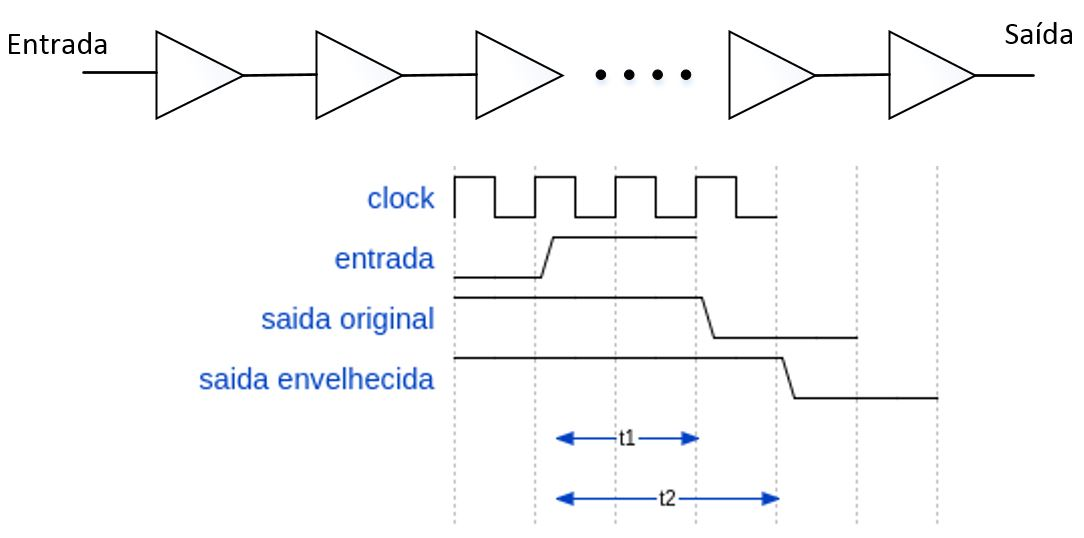
\includegraphics[width=0.8\textwidth]{images/output_delay}
	\caption{Variação no atraso de saída.}
	\label{figure:output_delay}
\end{figure}
Dado um tempo de propagação $t1$ como sendo o tempo necessário para que uma alteração na entrada seja percebida na saída de um circuito não-degradado e caso o tempo de propagação $t2$ medido após um tempo de operação $t_{oper}$ seja maior do que $t1$, este circuito será considerado como envelhecido, conforme exemplo mostrado na figura \ref{figure:output_delay}.

Assim, a variação do atraso de saída é considerada como:
\begin{equation}
\Delta t_d = t2 - t1
\label{eq:variacao_delay_saida}
\end{equation}

Idealmente este atraso de propagação não deveria aumentar. Entretanto, uma variação dele não é um fenômeno inesperado pelos projetistas. Por este motivo, uma salva-guarda (\textit{i.e.} guard-banding)  é planejada a nível de projeto.

Mesmo com esta medida, é possível que a degradação seja tal que extrapole essa salva-guarda. Dessa forma, a variação máxima do atraso $\Delta t_{d,max}$ não pode ultrapassar o \textit{guard-banding}.

\section{Tratamentos dos dados}
\label{section_tratamento_dados}
Os dados obtidos durante a extração de atrasos, MTTF e seus perfis correspondentes são aglutinados e populam o BDPE de forma definitiva. Estes dados compõe a base a ser usada como referência para os métodos descritos na seção \ref{section_metodos_estimativa}.

A formatação específica dessa informações a nível de software fica a critério do projetista. Além disso, o BDPE pode ser modificadp posteriormente para que novos perfis sejam adicionados.

Apesar de a metodologia não ser prejudicada pela existência de entradas duplicadas no banco de dados de perfis envelhecidos, é recomendado que as mesmas sejam únicas. Desta forma, o tamanho do BDPE é reduzido e consequentemente a quantidade de memória necessária para armazená-lo.

